\documentclass{beamer}
\usetheme{Madrid}
\usepackage{minted}
% sudo tlmgr install minted
\usepackage[utf8]{inputenc}
\usepackage[T2A]{fontenc}
\usepackage[russian,english]{babel}

% Footline: show current section (left) and frame numbers (right)
\setbeamertemplate{footline}{%
  \leavevmode%
  \hbox{%
    \begin{beamercolorbox}[wd=.78\paperwidth,ht=2.5ex,dp=1ex,left]{author in head/foot}%
      \hspace*{1em}\usebeamerfont{footline}\insertsectionhead%
    \end{beamercolorbox}%
    \begin{beamercolorbox}[wd=.22\paperwidth,ht=2.5ex,dp=1ex,right]{date in head/foot}%
      \usebeamerfont{footline}\insertframenumber{} / \inserttotalframenumber\hspace*{1em}%
    \end{beamercolorbox}%
  }%
}

\newcommand{\parpause}[1]{\only<+->{#1\par}}

\AtBeginSection[]
{
  \begin{frame}
    \frametitle{Содержание}
    \tableofcontents[currentsection]
  \end{frame}
}

\title{Семинар 1. Введение в распределенные системы}
\subtitle{Распределенные вычисления}
\author{Георгий Семенов}
\institute{Институт прикладных компьютерных наук \\ Университет ИТМО}
\date{весна 2026}

\begin{document}

\frame{\titlepage}

\begin{frame}
\frametitle{Домашние задания и оценивание}

\begin{itemize}
	\item По ходу курса будут появляться домашние задания с теорией и практикой – планируется $\approx 5$ заданий за весь курс.
	\item Оценка будет выставляться по результатам выполнения заданий (условия и детали появятся чуть позже).
	\item Как последняя возможность закрыться, будет экзамен (?), чтобы донабрать баллы.
\end{itemize}

\end{frame}

\begin{frame}
\frametitle{Где будет информация?}

\begin{itemize}
	\item Канал курса в Telegram (секция 'Практики')
	\item (скоро) Ссылка на репозиторий с материалами семинарских занятий и домашними заданиями
	\item (скоро) Таблица с баллами по домашним заданиям
\end{itemize}

\end{frame}

\begin{frame}
\frametitle{Литература и дополнительные материалы}

\begin{itemize}
	\item Готового полного списка для ознакомления - нет
	\item На семинарах / в домашних заданиях будем обращаться к литературе по необходимости
	\item В конце курса постараюсь поделиться подборкой, если захочется продолжить изучать темы
\end{itemize}

\end{frame}

\begin{frame}
\frametitle{О чем хочется поговорить на семинарах?}

(неупорядоченное множество)

\begin{itemize}
  \tiny
	\item Время и часики: реальное, векторные, Лампорта, другие кортежи; протоколы синхронизации времени
	\item Примеры архитектур распределенных систем и прикладных протоколов: DNS, CalDAV, SMB/CIFS и т.п.
  \item Немного повторить про сеть: OSI, TCP/UDP; брокеры сообщений (Kafka/RabbitMQ)
	\item Немного практического про Linux, Docker, Kubernetes, Ansible, Terraform
	\item Архитектуры: микросервисы, SOA
	\item Транспорт: RPC, Apache Thrift, gRPC, XML-RPC, JSON-RPC, Java RMI; CORBA, EJB
	\item Утверждения о 'невозможности' и модели согласованности: FLP-теорема, CAP-теорема, PACELC и т.п.
	\item Понятие консенсуса, консенсусное число, алгоритмы Paxos и Raft
	\item Пессимистическая и оптимистическая репликация: OT и CRDT (подробно на примерах)
	\item Распределенные файловые системы: NFS, GFS, BigTable, IPFS
	\item Распределенные блокировки, распределенные транзакции (Saga и т.п.)
	\item Инфраструктура больших данных и стриминг: MapReduce, Hadoop, Spark, YTsaurus
	\item Практический материал (пока не точно, посмотрим по делу): посмотрим на СУБД (Postgres, Mongo, Redis, HBase, Cassandra, Firebase), попробуем пописать инфраструктурные сервисы и скрипты (DNS?), порешать специфичные devops-задачи, потрогать Linux, запустить MapReduce-таску в Hadoop/YTsaurus
\end{itemize}

\end{frame}

\section{Что такое распределенные системы?}

\begin{frame}
  \frametitle{Определение}

  {\bfseries Распределенная система} – система связанных по сети компонентов – {\itshape узлов} (nodes), коммуницирующих
  и координирующих свои действия только с помощью отправки сообщений.

\end{frame}

\begin{frame}
  \frametitle{Некоторые трудности в распределенных системах}

  \begin{itemize}
    \item Конкурентность (concurrency) компонентов
      \begin{itemize}
        \item Геораспределенность узлов - издержки на обмен сообщениями по сети (время, деньги)
        \item Несколько узлов могут быть способны выполнить одну и ту же задачу, но без синхронизации они могут привести систему в несогласованное состояние
      \end{itemize}
    \item Отсутствие глобального времени
      \begin{itemize}
        \item На каждом узле своя система отсчета времени (CPU, RTC, ...)
        \item В связи с этим трудности установить точный порядок между действиями в системе
      \end{itemize}
    \item Независимые отказы компонентов
    \begin{itemize}
      \item Каждый узел может чисто статистически перестать работать (failure)
      \item Отдельный вид отказов, когда узел начинает работать неправильно или зловредно (byzantian failure)
    \end{itemize}
  \end{itemize}
\end{frame}

\begin{frame}
  \frametitle{Распределенные vs. высоконагруженные системы}

  {\bfseries Высоконагруженные системы} – те, что имеют {\itshape большую} пропускную способность (условно $> 10000$ RPS).

 \begin{itemize}
    \item Примеры распределенной и высоконагруженной системы
    \begin{itemize}
        \item DNS (Domain Name System) - core-технология для Web
        \item Всемирные социальные сети
        \item Поисковые системы
    \end{itemize}
    \item Примеры распределенной и НЕ высоконагруженной системы
    \begin{itemize}
        \item Внутренний git-сервер для небольшой компании
    \end{itemize}
    \item Примеры НЕ распределенной и высоконагруженной системы
    \begin{itemize}
        \item Монолитный бэкенд на одном мощном сервере
    \end{itemize}
  \end{itemize}

\end{frame}

\begin{frame}
  \frametitle{Распределенные vs. массивно параллельные системы}

 {\bfseries Массивно параллельные системы} – те, что используют {\itshape большое} количество
  вычислительных ядер/узлов одновременно (сотни, тысячи и более).

 \begin{itemize}
    \item Примеры распределенной и массивно параллельной системы
    \begin{itemize}
        \item Обработка данных на базе Apache Hadoop (MapReduce-кластеры)
        \item Apache Spark-кластеры для Big Data
        \item Обучение нейросетей в распределённом кластере GPU
    \end{itemize}

    \item Примеры распределенной и НЕ массивно параллельной системы
    \begin{itemize}
        \item Микросервисная архитектура с 5–10 сервисами
        \item Кластер базы данных с 3 репликами
    \end{itemize}

    \item Примеры НЕ распределенной и массивно параллельной системы
    \begin{itemize}
        \item HPC-приложение на одном сервере с 128 ядрами
        \item Программа, использующая GPU (CUDA) на одной машине
    \end{itemize}
  \end{itemize}

\end{frame}

\section{Немного о философии распределенных систем}

\begin{frame}
  \frametitle{Распределенность как направление мысли}

 \begin{itemize}
    \item Torrent-ы, блокчейн
    \begin{itemize}
        \item Технология как отражение прозрачного кооперативного экономического процесса
        \item Нерегулируемый способ решения прикладных задач
    \end{itemize}

    \item Децентрализованные социальные сети (Mastodon, Bluesky...)
    \begin{itemize}
        \item Переосмысление понятия свободы данных и приватности
        \item Локальность данных
    \end{itemize}

    \item Интернет вещей, роботы, умный дом, голосовые ассистенты
    \begin{itemize}
        \item Атрибуция интеллекта и знания в материальный объект
        \item Телевизор плохо ловит сигнал – ударим его тапком
        \item Распределенность как естественное свойство среды
        \item Что останется после нас, когда прилетят инопланетяне?
    \end{itemize}
  \end{itemize}

\end{frame}

\begin{frame}
  \frametitle{Понятие Local-First}

  {\bfseries Local-First} – философия разработки приложений, при которой
  данные в первую очередь хранятся и обрабатываются {\itshape локально} на устройстве пользователя,
  а синхронизация происходит асинхронно.

 \begin{itemize}
      \item Работа без постоянного подключения к сети (offline-first)
      \item Низкая задержка (нет round-trip к серверу)
      \item Пользователь контролирует свои данные
      \item Автоматическая синхронизация между устройствами
      \item Конфликт-устойчивость (CRDT, merge-алгоритмы)
  \end{itemize}
\end{frame}


\begin{frame}
  \frametitle{Mobile \& Ubiquitous Computing}

  {\bfseries Mobile computing} – вычисления, происходящие на мобильных устройствах,
  постоянно меняющих сеть, контекст и среду. \\

  {\bfseries Ubiquitous computing} (Mark Weiser) – идея «растворённых» вычислений,
  встроенных в окружающий мир. \\

 \begin{itemize}
    \item Множество устройств вместо одного компьютера
    \item Нестабильные сети и частичная связанность
    \item Данные распределены по физическому пространству
    \item Контекст-зависимость (локация, сенсоры, окружение)
    \item Вычисления становятся частью повседневной среды
  \end{itemize}
\end{frame}


\begin{frame}
  \frametitle{Философия распределённых систем — итог}

 \begin{itemize}
    \item Распределённость — это не только масштабирование,
          но и способ организации асинхронного взаимодействия

    \item Централизация $\rightarrow$ Кооперация между автономными агентами

    \item Единая точка истины $\rightarrow$ Согласование состояний
  \end{itemize}
  
\end{frame}


\section{Пример распределенной системы - DNS}

\begin{frame}
  \frametitle{Что такое DNS?}

  \begin{itemize}
    \item Domain Name System
    \item Иерархическое хранилище ресурсных записей (корневой узел - это точка)
    \item Протокол прикладного уровня (порт 53), который предоставляет для доменов - иерархических символьных единиц, различные записи:
    \begin{itemize}
      \item A - адрес IPv4
      \item AAAA - адрес IPv6
      \item CNAME - для переадресации на другой адрес
      \item MX - записи о почтовых серверах
      \item SRV - механизм service discovery (например, для сервера Minecraft)
      \item NS - адреса родительских DNS-серверов
      \item PTR - механизм обратной ссылки для поиска доменного имени по IP
    \end{itemize}
    \item Основное предназначение - трансляция доменов IP-адреса
  \end{itemize}

\end{frame}

\begin{frame}
  \frametitle{Сеть и OSI stack}

  \begin{center}
    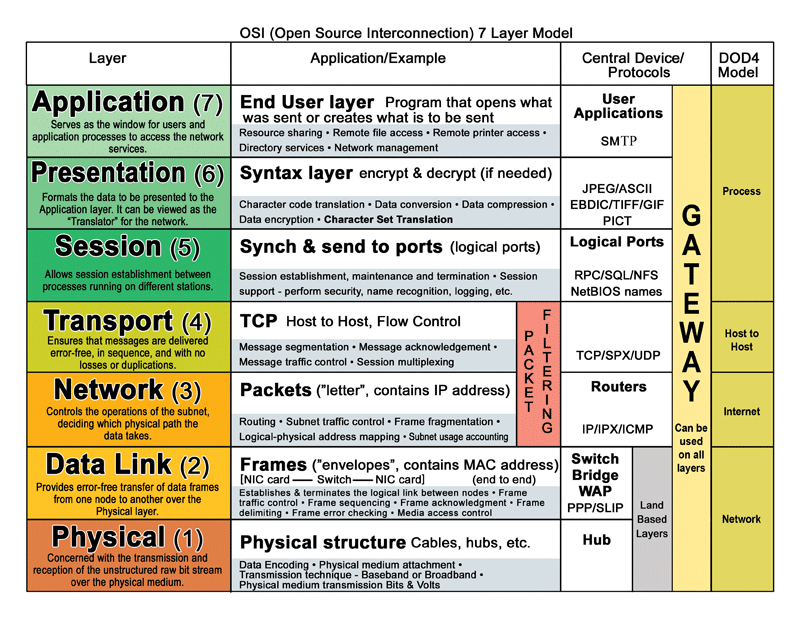
\includegraphics[width=0.9\linewidth,keepaspectratio]{images/OSI-Model.png}
  \end{center}

\end{frame}

\begin{frame}
  \frametitle{Иерархическое устройство DNS}

  \begin{center}
    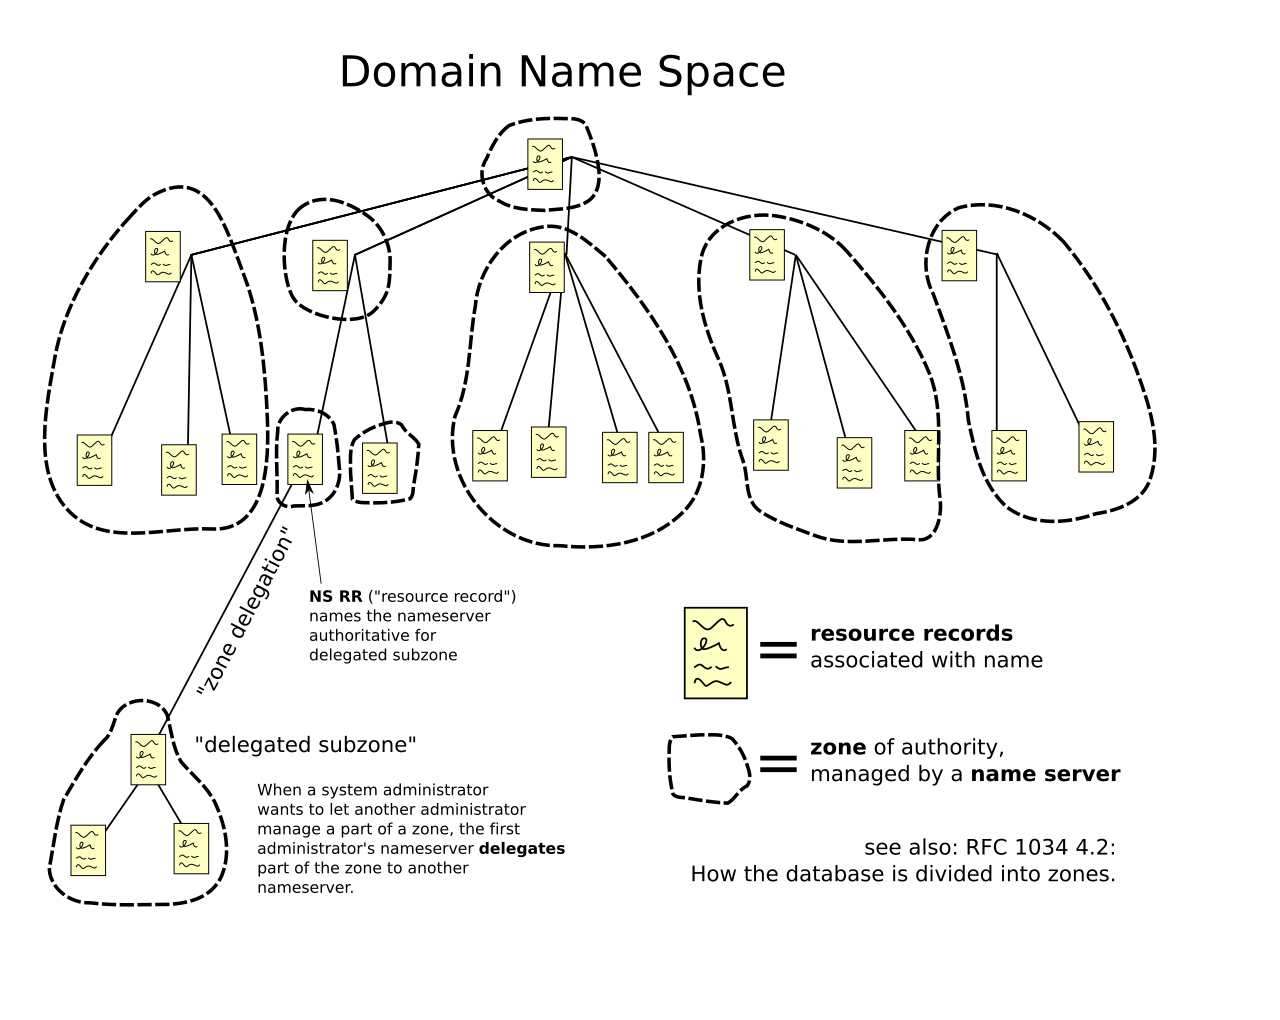
\includegraphics[width=0.9\linewidth,keepaspectratio]{images/Domain_name_space.svg}
  \end{center}

\end{frame}

\begin{frame}
  \frametitle{Сюжеты про DNS}

  \begin{itemize}
    \item Обеспечение высокой доступности данных и низкого времени отклика
    \item Естественная геораспределенность - национальные корневые зоны (например, .ru)
    \item Оптимистическая репликация (мягкое состояние - zone propogation) и TTL (time-to-live) у ресурсных записей
    \item Доменные регистраторы - как провайдеры управления доменными зонами
  \end{itemize}

\end{frame}

\begin{frame}
  \frametitle{Как попробовать DNS?}
  \begin{itemize}
    \item sudo apt install dnsutils
    \item dig example.com
    \item dig example.com MX
    \item dig @8.8.8.8 example.com
    \item dig +trace example.com
    \item dig +short example.com
  \end{itemize}
\end{frame}

\section{Время трогать траву в Minecraft: настраиваемся на DevOps}

\begin{frame}
  \frametitle{Почему Minecraft?}

  \begin{itemize}
    \item Мне просто есть, на чем показать, чтобы проговорить базовые понятия
    \item Пример архитектурной мысли для GameDev и для DevOps
    \item Firewall (закрываем/открываем портики, iptables): ufw status
    \item Docker / Docker Compose: мы договоримся о том, что понимаем, о чем идет речь
    \item Linux Services: systemctl list-units --type=service --state=running
  \end{itemize}

\end{frame}


\end{document}